\subsection{Документ <<Выработка гофроагрегата>>}
\label{doc:Doc_ProdGA}

% \subsubsection{Атрибуты}


% В документ необходимо добавить следующие колонки табличной части <<Раскрои>>.

% \pc
% \begin{longtable}{|p{4cm}|p{4cm}|p{8cm}|}
% \hline
% {\bf Наименование} & {\bf Тип данных} &  {\bf Комментарий} \endhead
%     \hline
%     Менеджер & Справочник <<Физические лица>> & Менеджер, который создал заказ на выпуск данного изделия. Подтягивается из заявки текущего заказа. Закрыто для редактирования.\\
%     \hline
%     Номер связки & Число (10,0) & Номер связки раскроя для выгрузки в память гофроагрегата.\\
%     \hline   
%    \caption{Новые колонки табличной части <<Раскрои>>}
%   \label{tab:ProdGA}
% \end{longtable}

\subsubsection{Функциональные требования}

\point{Изменить форму документа}

Добавить группу команд по связи с гофроагрегатом.
Добавить в группу индикатор состояния подключения к гофроагрегату.
При положительном подключении индикатор после выполнения команды НачатьЧтениеДанныхГА должен показывать статус подключения к ГА.
При отрицательном подключении индикатор должен показывать красный сигнал ошибки.

Форма редактирования документа представлена на рисунке \ref{fig:placeholder}.
\begin{figure}[h]
    \centering
    \fbox{
    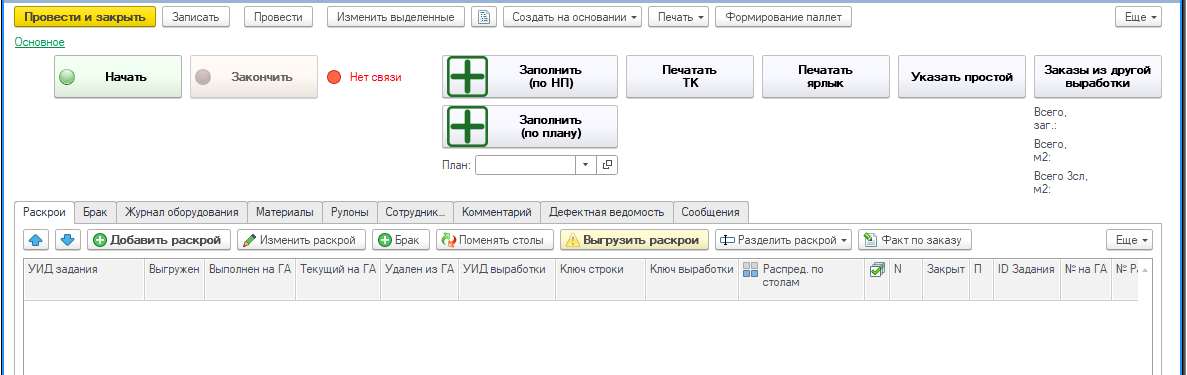
\includegraphics[height=0.21 \textheight, keepaspectratio]{50_Pics/Doc_ProdGA.png}}
    \caption{Измененная форма редактирования документа}
    \label{fig:placeholder}
\end{figure}


\point{Добавить команду ''Выгрузить раскрои''}

В документе <<Выработка гофроагрегата>> в табличной части <<Раскрои>> добавить команду ''Выгрузить раскрои''.
Выделенные пользователем в табличной части ''Раскрои'' должны быть по команде выгружены в память гофроагрегата JSM.
Для выгруженного задания должен быть указан признак ''Выгружен'' Истина.
При повторной выгрузке задание не должно быть выгружено без удаления на стороне JSM.


\point{Добавить команду ''Начать чтение данных ГА''}

По команде система должна начать считывать данные с ГА согласно функции \ref{sec:startreading} ''Начать чтение данных с ГА''. Статус подключения должен измениться на ''Подключен''.


\point{Добавить команду ''Закончить чтение данных ГА''}

По команде система должна закончить считывать данные с ГА согласно функции \ref{sec:stopreading} ''Закончить чтение данных с ГА''. Статус подключения должен измениться на ''Нет связи''.


